\documentclass[a4paper]{article}
\usepackage{graphicx}
\usepackage[a4paper, margin=2cm]{geometry}
\setlength{\parindent}{0pt}

\title{Lab 4 - Report}
\author{rayane guerou}

\begin{document}

\maketitle

\section{GPU greyscale}
We firstly import an image with matplotlib that is represented as a ndarray in shape of (imageHeight, imageWidth, 3).
Now Instead of flatting the image like in the lab3, We've used 2D array of channels to represent the image.

\begin{figure}[h!]
\centering
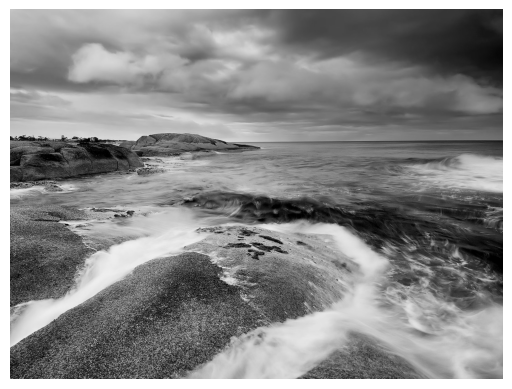
\includegraphics[scale=0.5]{src/gpu1d.png}
\caption{GPU greyscale 1d}
\end{figure}

\begin{figure}[h!]
    \centering
    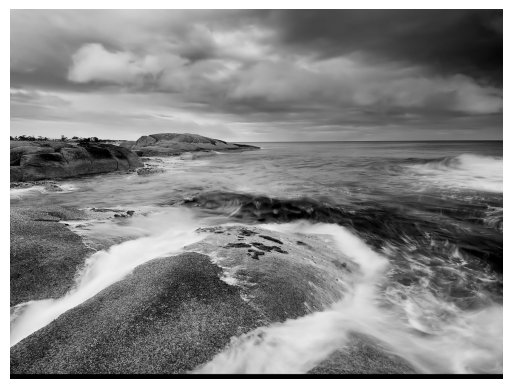
\includegraphics[scale=0.5]{src/gpu2d.png}
    \caption{GPU greyscale 2d}
\end{figure}

We can see that the 2d grayscale is more faster than the 1d method

\end{document}
